\showchapterboxtrue 
\mychapter{Mechanics}


\section{Topology and Mobility Analysis}
\subsection{Exercise 1}
In this exercise, we will analyze the topology and mobility of two different robot configurations: a 6-DOF serial robot and a parallel robot (Stewart platform). Figure \ref{fig:robotcomparison} shows a comparison of these two types of robots.

\begin{figure}[H]
    \centering
    \begin{subfigure}[]{0.45\textwidth}
        \centering
        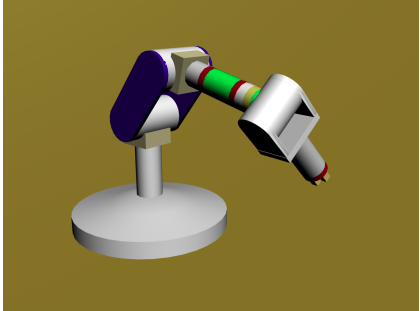
\includegraphics[width=\textwidth]{6DofSerialRobot}
        \caption{6-DOF Serial Robot}
        \label{fig:6dofserialrobot}
    \end{subfigure}
    \hfill
    \begin{subfigure}[]{0.35\textwidth}
        \centering
        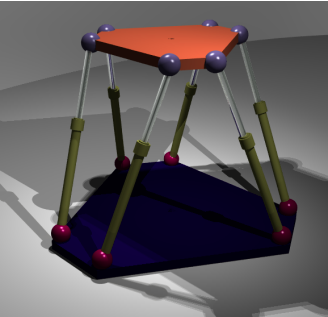
\includegraphics[width=\textwidth]{ParallelRobot}
        \caption{Parallel Robot}
        \label{fig:parallelrobot}
    \end{subfigure}
    \caption{Comparison of 6-DOF Serial Robot and Parallel Robot}
    \label{fig:robotcomparison}
\end{figure}




Let's start by analyzing the 6-DOF serial robot in more detail. Figure \ref{fig:6dofserial} illustrates the joint axes and links of this robot.

\begin{figure}[H]
    \centering
    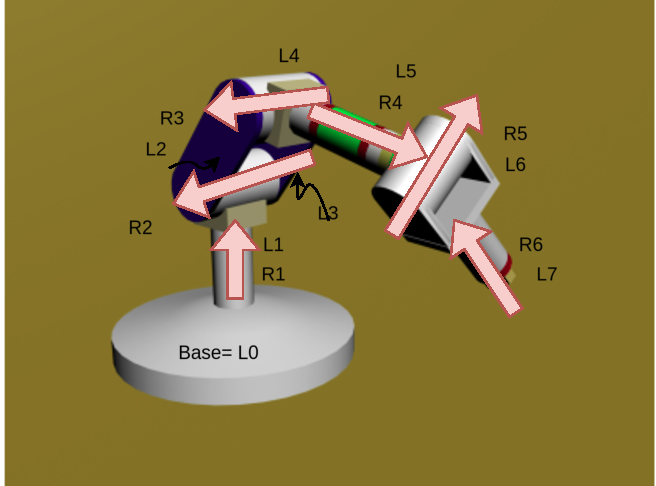
\includegraphics[width=0.45\textwidth]{6dofserial.pdf}
    \caption{Joint axes and links of the 6-DOF serial robot}
    \label{fig:6dofserial}
\end{figure}


\begin{solution}[8-Link Serial Robot]
    The serial robot described in Figure \ref{fig:6dofserialrobot} and detailed in Figure \ref{fig:6dofserial} is a typical example of an industrial robotic arm. It consists of the following components:

\begin{itemize}
    \item \textbf{Base (L\textsubscript{0})}: 
    \begin{itemize}
        \item This is the fixed part of the robot, usually mounted on the ground or a stable platform.
        \item It serves as the reference frame for the entire robot structure.
    \end{itemize}
    
    \item \textbf{Seven Moving Links (L\textsubscript{1} to L\textsubscript{7})}:
    \begin{itemize}
        \item These are the rigid bodies that make up the robot's arm.
        \item Each link connects to the next via a joint, forming a chain-like structure.
        \item L\textsubscript{7} is typically the end-effector or the link to which a tool or gripper is attached.
    \end{itemize}
    
    \item \textbf{Revolute Joints (J\textsubscript{0} to J\textsubscript{6})}:
    \begin{itemize}
        \item These joints connect the links and allow rotational motion between them.
        \item Each joint has one degree of freedom, allowing rotation around a single axis.
        \item The joints are typically labeled J\textsubscript{0}, J\textsubscript{1}, J\textsubscript{2}, J\textsubscript{3}, J\textsubscript{4}, J\textsubscript{5}, and J\textsubscript{6}.
    \end{itemize}
    
    \item \textbf{Connectivity}:
    \begin{itemize}
        \item Base (L\textsubscript{0}) is connected to L\textsubscript{1} via J\textsubscript{0}
        \item L\textsubscript{1} is connected to L\textsubscript{2} via J\textsubscript{1} and to L\textsubscript{3} via J\textsubscript{2}
        \item L\textsubscript{2} is connected to L\textsubscript{4} via J\textsubscript{3}
        \item L\textsubscript{3} is connected to L\textsubscript{4} via J\textsubscript{4}
        \item L\textsubscript{4} is connected to L\textsubscript{5} via J\textsubscript{5}
        \item L\textsubscript{5} is connected to L\textsubscript{6} via J\textsubscript{6}
        \item L\textsubscript{6} is connected to L\textsubscript{7} via J\textsubscript{7}
    \end{itemize}
    
    \item \textbf{Kinematic Chain}:
    \begin{itemize}
        \item The robot forms an open kinematic chain, starting from the base and ending at the end-effector.
        \item Each joint adds one degree of freedom to the robot.
    \end{itemize}
    
    \item \textbf{Degrees of Freedom}:
    \begin{itemize}
        \item With seven revolute joints, this robot has 7 degrees of freedom (7-DOF).
        \item This allows the end-effector to achieve any position and orientation within its workspace.
    \end{itemize}
\end{itemize}

 \subsection*{Connectivity Graph}

Based on Featherstone's \cite{featherstone2014rigid} definition, the connectivity graph for this robot represents each link as a node and each joint as an edge connecting the nodes, clearly showing the serial nature of the robot's structure with parallel connections.

\begin{figure}[H]
    \centering
    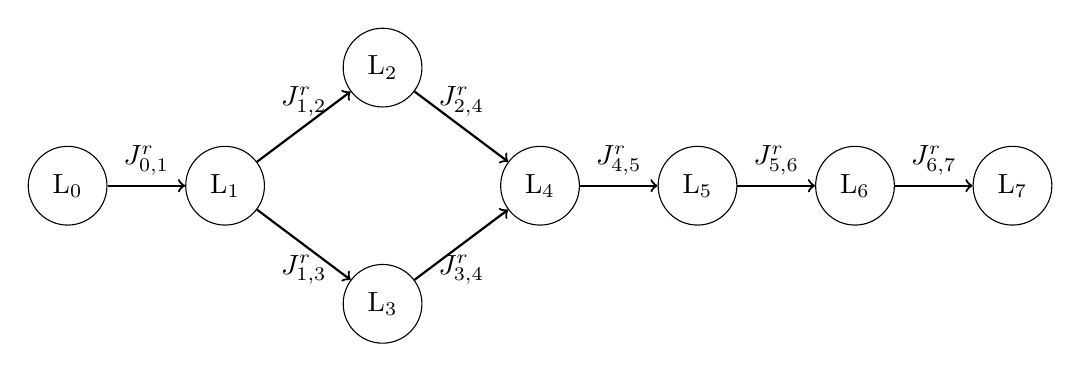
\begin{tikzpicture}[node distance=2cm and 1.5cm, 
        block/.style={circle, draw, minimum size=1cm},
        line/.style={->, thick}]
        
        % Nodes (Links)
        \node[block, fill=white] (L0) at (0,0) {L\textsubscript{0}};
        \node[block] (L1) at (2,0) {L\textsubscript{1}};
        \node[block] (L2) at (4,1.5) {L\textsubscript{2}};
        \node[block] (L3) at (4,-1.5) {L\textsubscript{3}};
        \node[block] (L4) at (6,0) {L\textsubscript{4}};
        \node[block] (L5) at (8,0) {L\textsubscript{5}};
        \node[block] (L6) at (10,0) {L\textsubscript{6}};
        \node[block] (L7) at (12,0) {L\textsubscript{7}};
        
        % Arcs (Joints)
        \draw[line] (L0) -- (L1) node[midway, above] {$J^r_{0,1}$};
        \draw[line] (L1) -- (L2) node[midway, above] {$J^r_{1,2}$};
        \draw[line] (L1) -- (L3) node[midway, below] {$J^r_{1,3}$};
        \draw[line] (L2) -- (L4) node[midway, above] {$J^r_{2,4}$};
        \draw[line] (L3) -- (L4) node[midway, below] {$J^r_{3,4}$};
        \draw[line] (L4) -- (L5) node[midway, above] {$J^r_{4,5}$};
        \draw[line] (L5) -- (L6) node[midway, above] {$J^r_{5,6}$};
        \draw[line] (L6) -- (L7) node[midway, above] {$J^r_{6,7}$};
    \end{tikzpicture}
    \caption{Connectivity graph for an 8-link serial robot with parallel connections}
    \label{fig:connectivity_graph}
\end{figure}

In this topological graph:
\begin{itemize}
    \item Nodes (circles) represent links L\textsubscript{0} to L\textsubscript{7}.
    \item Edges (arrows) represent joints J\textsubscript{0} to J\textsubscript{7}.
    \item The white node (L\textsubscript{0}) represents the fixed base.
    \item The graph clearly shows the serial chain structure of the robot with parallel connections.
\end{itemize}
\end{solution}

\begin{solution}[Connectivity graph for the 6-SPS parallel robot (Stewart platform)]
    Now, let's analyze the connectivity of the parallel robot (Stewart platform) shown in Figure \ref{fig:parallelrobot}. Figure \ref{fig:connectivity_graph_6sps_detailed} illustrates the connectivity graph for this 6-SPS parallel robot.
\begin{figure}[H]
	\centering
	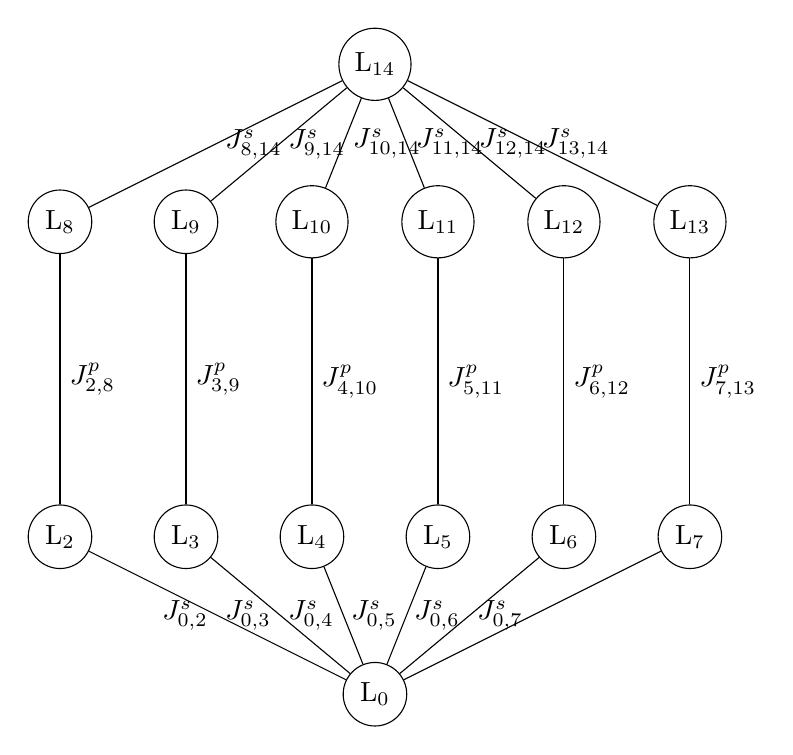
\begin{tikzpicture}[
	node distance=2cm,
	block/.style={circle, draw, minimum size=0.8cm},
	line/.style={-}
	]
	% Base and Top platform
	\node[block, fill=white] (L0) at (0,-4) {L\textsubscript{0}};
	\node[block] (L1) at (0,4) {L\textsubscript{14}};
	
	% First layer of legs
	\node[block] (L2) at (-4,-2) {L\textsubscript{2}};
	\node[block] (L3) at (-2.4,-2) {L\textsubscript{3}};
	\node[block] (L4) at (-0.8,-2) {L\textsubscript{4}};
	\node[block] (L5) at (0.8,-2) {L\textsubscript{5}};
	\node[block] (L6) at (2.4,-2) {L\textsubscript{6}};
	\node[block] (L7) at (4,-2) {L\textsubscript{7}};
	
	% Second layer of legs
	\node[block] (L8) at (-4,2) {L\textsubscript{8}};
	\node[block] (L9) at (-2.4,2) {L\textsubscript{9}};
	\node[block] (L10) at (-0.8,2) {L\textsubscript{10}};
	\node[block] (L11) at (0.8,2) {L\textsubscript{11}};
	\node[block] (L12) at (2.4,2) {L\textsubscript{12}};
	\node[block] (L13) at (4,2) {L\textsubscript{13}};
	
	% Connections
	\foreach \i/\j in {2/8,3/9,4/10,5/11,6/12,7/13} {
		\draw[line] (L0) -- (L\i) node[midway, left] {$J^s_{0,\i}$};
		\draw[line] (L\i) -- (L\j) node[midway, right] {$J^p_{\i,\j}$};
		\draw[line] (L\j) -- (L1) node[midway, right] {$J^s_{\j,14}$};
	}
	\end{tikzpicture}
	\caption{Connectivity graph for the 6-SPS parallel robot (Stewart platform)}
	\label{fig:connectivity_graph_6sps_detailed}
\end{figure}

\begin{description}
	\item[Connectivity Graph:] The graph represents the structure of a 6-SPS (Spherical-Prismatic-Spherical) parallel robot, also known as a Stewart platform.
	
	\item \textbf{Components:}
	\begin{itemize}
		\item \textbf{Base (L\textsubscript{0}):} Represented by the white node at the bottom.
		\item \textbf{End-Effector (L\textsubscript{14}):} Represented by the top node, it's the moving platform.
		\item \textbf{Legs:} Six kinematic chains, each composed of two links:
		\begin{itemize}
			\item Lower links: L\textsubscript{2} to L\textsubscript{7}
			\item Upper links: L\textsubscript{8} to L\textsubscript{13}
		\end{itemize}
	\end{itemize}
	
	\item \textbf{Joints:}
	\begin{itemize}
		\item \textbf{Spherical Joints (S):} 
		\begin{itemize}
			\item Base to lower links: $J^s_{0,i}$ where $i = 2, 3, ..., 7$
			\item Upper links to End-Effector: $J^s_{j,14}$ where $j = 8, 9, ..., 13$
		\end{itemize}
		\item \textbf{Prismatic Joints (P):} 
		\begin{itemize}
			\item Between lower and upper links: $J^p_{i,j}$ where $i = 2, 3, ..., 7$ and $j = i+6$
		\end{itemize}
	\end{itemize}
	
	\item[Structure:] Each of the six legs follows an SPS (Spherical-Prismatic-Spherical) configuration, connecting the base to the end-effector. This arrangement provides the robot with 6 degrees of freedom (3 translational and 3 rotational).
\end{description}
\end{solution}





\subsection{Exercise 2}
\addcontentsline{toc}{subsection}{Exercise 2}

The Chebyshev–Grübler–Kutzbach criterion estimates the degree of freedom (DOF) of a kinematic chain, that is, a coupling of rigid bodies by means of mechanical constraints. The general mobility of a robot can be estimated by the following criteria \cite{taghirad2013parallel}:

\begin{equation}
    F = \lambda(n - j - 1) + \sum_{i=1}^j f_i - f_p,
    \label{eq:cgk_extended}
\end{equation}

where
\begin{itemize}
    \item $F$ – degrees-of-freedom of the mechanism
    \item $\lambda$ – degree-of-freedom of the space (= 3 for planar and spherical mechanisms, = 6 for spatial mechanisms)
    \item $n$ – number of links in the mechanism including the base
    \item $j$ – number of binary joints of the mechanism
    \item $f_i$ – degrees of relative motion permitted by joint $i$
    \item $f_p$ – total number of passive degrees-of-freedom
\end{itemize}

\begin{solution}
    Let's compute the mobility of the two robots shown in Figure \ref{fig:robotcomparison} using Equation \ref{eq:cgk_extended}.

    \subsection*{1. 6-DOF Serial Robot}
    For the serial robot (Figure \ref{fig:6dofserialrobot}):
    \begin{itemize}
        \item $\lambda = 6$ (spatial mechanism)
        \item $n = 8$ (7 moving links + 1 base)
        \item $j = 7$ (7 revolute joints)
        \item $\sum_{i=1}^j f_i = 7$ (1 DOF per revolute joint)
        \item $f_p = 0$ (no passive degrees-of-freedom)
    \end{itemize}

    Applying Equation \ref{eq:cgk_extended}:
    \begin{align*}
        F &= \lambda(n - j - 1) + \sum_{i=1}^j f_i - f_p \\
          &= 6(8 - 7 - 1) + 7 - 0 \\
          &= 6(0) + 7 \\
          &= 7
    \end{align*}

    The mobility of the 6-DOF serial robot is 7, which matches our earlier analysis.

    \subsection*{2. 6-SPS Parallel Robot (Stewart Platform)}
    For the parallel robot (Figure \ref{fig:parallelrobot}):
    \begin{itemize}
        \item $\lambda = 6$ (spatial mechanism)
        \item $n = 14$ (12 leg links + 1 base + 1 platform)
        \item $j = 18$ (12 spherical joints + 6 prismatic joints)
        \item $\sum_{i=1}^j f_i = 42$ (3 DOF per spherical joint × 12 + 1 DOF per prismatic joint × 6)
        \item $f_p = 6$ (1 passive DOF per leg, rotating around its axis)
    \end{itemize}

    Applying Equation \ref{eq:cgk_extended}:
    \begin{align*}
        F &= \lambda(n - j - 1) + \sum_{i=1}^j f_i - f_p \\
          &= 6(14 - 18 - 1) + 42 - 6 \\
          &= 6(-5) + 42 - 6 \\
          &= -30 + 42 - 6 \\
          &= 6
    \end{align*}

    The calculated mobility of the 6-SPS parallel robot is 6, which is correct.

    \subsection*{Simplified Formula for Serial Robots}
    For serial robots, we can simplify Equation \ref{eq:cgk_extended} because:
    \begin{itemize}
        \item The number of joints is always one less than the number of links ($j = n - 1$)
        \item There are typically no passive degrees-of-freedom ($f_p = 0$)
    \end{itemize}

    Substituting these into Equation \ref{eq:cgk_extended}:
    \begin{align*}
        F &= \lambda(n - j - 1) + \sum_{i=1}^j f_i - f_p \\
          &= \lambda(n - (n-1) - 1) + \sum_{i=1}^j f_i - 0 \\
          &= \lambda(0) + \sum_{i=1}^j f_i \\
          &= \sum_{i=1}^j f_i
    \end{align*}

    Therefore, the simplified formula for serial robots is:
    \begin{equation}
        F = \sum_{i=1}^j f_i
        \label{eq:serial_mobility}
    \end{equation}

    This means that for serial robots, the mobility is simply the sum of the degrees of freedom of all joints.

    \subsection*{Application to Parallel Mechanisms}
    The extended Chebyshev–Grübler–Kutzbach criterion (Equation \ref{eq:cgk_extended}) works accurately for parallel mechanisms when we account for passive degrees-of-freedom. In the case of the Stewart platform:

    1. Each spherical joint contributes 3 DOF to $\sum_{i=1}^j f_i$.
    2. Each prismatic joint contributes 1 DOF to $\sum_{i=1}^j f_i$.
    3. Each leg has 1 passive DOF (rotation around its axis), contributing to $f_p$.

    By including these passive degrees-of-freedom in our calculation, we obtain the correct mobility of 6 for the Stewart platform without needing additional simplifications or corrections.

    This demonstrates the importance of considering passive degrees-of-freedom when analyzing the mobility of complex parallel mechanisms.
\end{solution}


\subsection{Exercise 3}
\addcontentsline{toc}{subsection}{Exercise 3}

It seems almost magical that a simple formula like the Chebychev–Grübler–Kutzbach criterion can be used to estimate the general mobility of a system. Does it always work? Can you find some counter-examples where this formula fails?

\begin{solution}
	
    While the Chebychev–Grübler–Kutzbach criterion is a powerful tool for estimating the mobility of many mechanical systems, it does not always work correctly. This paper \cite{gogu2005chebychev} addresses most of mechanisms that the mobility criteria failed to predict their DOF. Here we state  several situations where the formula can fail to accurately predict the degrees of freedom of a mechanism. Let's explore some of these cases:

    \subsection*{1. Overconstrained Mechanisms}
    Some mechanisms are overconstrained yet still mobile due to special geometric conditions. The Chebychev–Grübler–Kutzbach criterion often predicts zero or negative mobility for these systems, even though they can move.

	

    \textbf{Example: Bennett's Linkage}
    \begin{figure}[H]
        \centering
        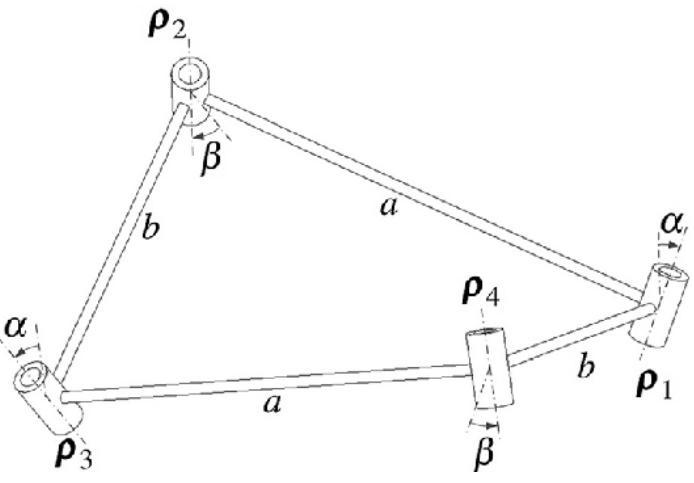
\includegraphics[width=0.5\textwidth]{The-Bennett-linkage-and-its-geometric-description-22_Q640.jpg}
        \caption{Bennett's Linkage \cite{lu2017approximation}}
        \label{fig:bennett_linkage}
    \end{figure}

    Bennett's linkage is a spatial 4-bar linkage with one degree of freedom. However, applying the Chebychev–Grübler–Kutzbach criterion:

    \begin{itemize}
        \item $\lambda = 6$ (spatial mechanism)
        \item $n = 4$ (4 links)
        \item $j = 4$ (4 revolute joints)
        \item $\sum_{i=1}^j f_i = 4$ (1 DOF per revolute joint)
        \item $f_p = 0$ (no passive DOF)
    \end{itemize}

    \begin{align*}
        F &= \lambda(n - j - 1) + \sum_{i=1}^j f_i - f_p \\
          &= 6(4 - 4 - 1) + 4 - 0 \\
          &= 6(-1) + 4 \\
          &= -2
    \end{align*}

    The formula predicts -2 DOF, but the mechanism actually has 1 DOF due to its special geometry.

    \subsection*{2. Mechanisms with Redundant Constraints}
    Some mechanisms have redundant constraints that don't affect mobility but are counted in the formula.

    \textbf{Example: Parallel Manipulator with Redundant Actuation}
    Consider a planar parallel manipulator with three legs, each containing an actuated prismatic joint, where only two actuators are needed for full mobility.
    
    \begin{figure}[H]
        \centering
        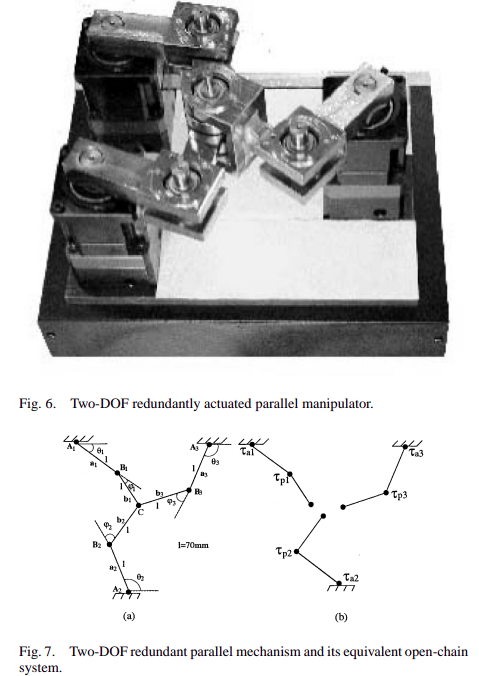
\includegraphics[width=0.5\textwidth]{redudant.png}
        \caption{Two-DOF redundantly actuated parallel manipulator \cite{cheng2003dynamics}}
        \label{fig:redundant_parallel}
    \end{figure}

    Applying the formula:
    \begin{itemize}
        \item $\lambda = 3$ (planar mechanism)
        \item $n = 8$ (1 base, 1 platform, 6 leg links)
        \item $j = 9$ (3 prismatic + 6 revolute joints)
        \item $\sum_{i=1}^j f_i = 9$ (1 DOF per joint)
        \item $f_p = 0$ (no passive DOF)
    \end{itemize}

    \begin{align*}
        F &= \lambda(n - j - 1) + \sum_{i=1}^j f_i - f_p \\
          &= 3(8 - 9 - 1) + 9 - 0 \\
          &= 3(-2) + 9 \\
          &= 3
    \end{align*}

    The formula predicts 3 DOF, which is correct, but it doesn't account for the redundant actuation.

    \subsection*{3. Mechanisms with Special Configurations}
    Some mechanisms can change their mobility in certain configurations, which the formula doesn't capture.

    \textbf{Example: Bricard's Flexible Octahedron \cite{baker1980analysis}} :
    This mechanism can transition between 0 and 1 DOF depending on its configuration, but the Chebychev–Grübler–Kutzbach criterion always predicts the same mobility.

    \subsection*{4. Mechanisms with Higher Pair Joints}
    The formula assumes lower pair joints (e.g., revolute, prismatic). It may not accurately predict mobility for mechanisms with higher pair joints (e.g., cam-follower systems).

    \subsection*{Conclusion}
    While the Chebychev–Grübler–Kutzbach criterion is a valuable tool for initial mobility analysis, it has limitations. It's important to consider:

    \begin{itemize}
        \item Special geometric conditions
        \item Redundant constraints
        \item Configuration-dependent mobility
        \item The nature of the joints involved
    \end{itemize}

    In complex or unusual mechanisms, additional analysis methods (e.g., screw theory, instantaneous kinematics) may be necessary to accurately determine mobility.
\end{solution}

\section{Geometry and Kinematics}
\subsection{Exercise 4}


A serially connected 3 DOF robotic leg with 2 orthogonally intersecting revolute joints and a 1 DOF prismatic joint is shown in Figure \ref{fig:3dof_robotic_leg}. Given $q_1$ and $q_2$ denote the joint angles in the first two revolute joints and $q_3$ denote the linear displacement in the prismatic joint:

\begin{figure}[H]
	\centering
	
\includegraphics[width=0.3\textwidth]{3dofUP.pdf}
	\caption{A 3 DOF robotic leg with 2 revolute and 1 prismatic joints}
	\label{fig:3dof_robotic_leg}
\end{figure}

\begin{solution}
	
	\subsection*{1. Geometric object where the end-effector point E lives}
	
	The end-effector point E lives in a three-dimensional Euclidean space, $\mathbb{R}^3$. More specifically, it traces out a subset of $\mathbb{R}^3$ that forms the workspace of the robot.
	
	\subsection*{2. Forward Kinematics using Product of Exponentials (PoE)} \label{sec:SE3}

Based on Kevin-Lynch's Modern Robotics book \cite{lynch2017modern} the forward kinematics for our 3 DOF robotic leg can be derived using the Product of Exponentials (PoE) formula. This method offers an elegant and intuitive approach, particularly suitable for open kinematic chains like our robot leg. Let's go through the process step-by-step:

\subsubsection*{Step 1: Define Frames}
\begin{itemize}
    \item \textbf{Space Frame \{s\}}: Fixed at the base of the robot.
    \item \textbf{Body Frame \{b\}}: Attached to the end-effector (point E).
\end{itemize}

\subsubsection*{Step 2: Zero Configuration}
Set all joint variables $(q_1, q_2, q_3)$ to zero. In this configuration, the transformation matrix $M \in SE(3)$ from \{s\} to \{b\} is:

\begin{equation}
    M = \begin{bmatrix}
    1 & 0 & 0 & 0 \\
    0 & 1 & 0 & 0 \\
    0 & 0 & 1 & L_0 \\
    0 & 0 & 0 & 1
    \end{bmatrix}
\end{equation}

\subsubsection*{Step 3: Determine Screw Axes}
For our robot, we need to determine the screw axes for each joint $(\omega_i^T , v_i^T)^T $. The screw axis is represented by two vectors: $\omega_i$ (axis of rotation or translation) and $v_i$ (linear velocity). Let's examine how we calculate $v_i$ for each type of joint:

\paragraph{Revolute Joints (Joints 1 and 2):}
For a revolute joint, $v_i$ is calculated using the formula:

\begin{equation}
v_i = -\omega_i \times q_i
\end{equation}

where $q_i$ is any point on the joint axis. This formula comes from the fact that the linear velocity of any point on a rigid body rotating about an axis is given by the cross product of the angular velocity vector and the position vector from any point on the axis to the point in question.

\begin{itemize}
	\item \textbf{Joint 1:} The axis of rotation is along the y-axis, passing through the origin.
	\begin{align*}
	\omega_1 &= [0, 1, 0]^T \\
	q_1 &= [0, 0, 0]^T \text{ (we can choose the origin as our point)} \\
	v_1 &= -\omega_1 \times q_1 = -[0, 0, 1]^T \times [0, 0, 0]^T = [0, 0, 0]^T
	\end{align*}
	
	\item \textbf{Joint 2:} The axis of rotation is along the x-axis, passing through the origin $[0, 0, 0]$.
	\begin{align*}
	\omega_2 &= [1, 0, 0]^T \\
	q_2 &= [0, 0, 0]^T \\
	v_2 &= -\omega_2 \times q_2 = -[1, 0, 0]^T \times [0, 0, 0]^T = [0, 0, 0]^T
	\end{align*}
\end{itemize}

\paragraph{Prismatic Joint (Joint 3):}
For a prismatic joint, $\omega_i$ is zero (no rotation), and $v_i$ is simply a unit vector in the direction of positive translation.

\begin{itemize}
	\item \textbf{Joint 3:} The prismatic joint moves along the z-axis of the space frame after the second rotation.
	\begin{align*}
	\omega_3 &= [0, 0, 0]^T \\
	v_3 &= [0, 0, 1]^T \text{ (unit vector in the direction of translation)}
	\end{align*}
\end{itemize}

This calculation of $v_i$ ensures that the screw axis correctly represents the motion of each joint, whether it's a rotation around an axis (revolute) or a translation along an axis (prismatic).

\subsubsection*{Step 4: Screw Axis Matrices (Extended Explanation)}

In the Product of Exponentials (PoE) formula, we represent each joint's motion using a 4x4 matrix $[S_i] \in se(3)$, where $se(3)$ is the Lie algebra of the Special Euclidean group SE(3). This matrix encapsulates both the rotational and translational components of the joint's motion.

The general form of the screw axis matrix $[S_i]$ is:

\begin{equation}
[S_i] = \begin{bmatrix}
[\omega_i] & v_i \\
0 & 0
\end{bmatrix}
\end{equation}

where $[\omega_i]$ is the 3x3 skew-symmetric matrix representation of $\omega_i$, and $v_i$ is the 3x1 linear velocity vector we calculated in Step 3.

For a vector $\omega = [\omega_1, \omega_2, \omega_3]^T$, its skew-symmetric matrix representation is:

\begin{equation}
[\omega] = \begin{bmatrix}
0 & -\omega_3 & \omega_2 \\
\omega_3 & 0 & -\omega_1 \\
-\omega_2 & \omega_1 & 0
\end{bmatrix}
\end{equation}

Now, let's calculate $[S_i]$ for each joint:

\paragraph{Joint 1 (Revolute):}
$\omega_1 = [0, 1, 0]^T$, $v_1 = [0, 0, 0]^T$

\begin{equation}
[S_1] = \begin{bmatrix}
0 & 0 & 1 & 0 \\
0 & 0 & 0 & 0 \\
-1 & 0 & 0 & 0 \\
0 & 0 & 0 & 0
\end{bmatrix}
\end{equation}

\paragraph{Joint 2 (Revolute):}
$\omega_2 = [1, 0, 0]^T$, $v_2 = [0, 0, 0]^T$

\begin{equation}
[S_2] = \begin{bmatrix}
0 & 0 & 0 & 0 \\
0 & 0 & -1 & 0 \\
0 & 1 & 0 & 0 \\
0 & 0 & 0 & 0
\end{bmatrix}
\end{equation}

\paragraph{Joint 3 (Prismatic):}
$\omega_3 = [0, 0, 0]^T$, $v_3 = [0, 0, 1]^T$

\begin{equation}
[S_3] = \begin{bmatrix}
0 & 0 & 0 & 0 \\
0 & 0 & 0 & 0 \\
0 & 0 & 0 & 1\\
0 & 0 & 0 & 0
\end{bmatrix}
\end{equation}

\paragraph{Interpretation:}
- For revolute joints (1 and 2), the upper-left 3x3 submatrix represents the axis of rotation, while the upper-right 3x1 vector represents the moment of the axis.
- For the prismatic joint (3), the upper-left 3x3 submatrix is zero

\subsubsection*{Step 5: PoE Formula}
The forward kinematics is given by:

\begin{equation}
    T(q_1, q_2, q_3) = e^{[S_1]q_1} e^{[S_2]q_2} e^{[S_3]q_3} M
\end{equation}

\subsubsection*{Step 6: Compute Matrix Exponentials}
\begin{align*}
    e^{[S_1]q_1} &= \begin{bmatrix}
    \cos q_1 & 0 & \sin q_1 & 0 \\
    0 & 1 & 0 & 0 \\
    -\sin q_1 & 0 & \cos q_1 & 0 \\
    0 & 0 & 0 & 1
    \end{bmatrix} \\
    e^{[S_2]q_2} &= \begin{bmatrix}
    1 & 0 & 0 & 0 \\
    0 & \cos q_2 & -\sin q_2 & 0 \\
    0 & \sin q_2 & \cos q_2 & 0 \\
    0 & 0 & 0 & 1
    \end{bmatrix} \\
    e^{[S_3]d} &= \begin{bmatrix}
    1 & 0 & 0 & 0 \\
    0 & 1 & 0 & 0 \\
    0 & 0 & 1 & d \\
    0 & 0 & 0 & 1
    \end{bmatrix}
\end{align*}

\subsubsection*{Step 7: Final Forward Kinematics}
Multiplying these matrices together, we get the final transformation:

\begin{equation}
    T(q_1, q_2, q_3) = \begin{bmatrix}
    \cos q_1 & \sin q_1 \sin q_2 & \sin q_1 \cos q_2 & \cos q_2 \sin q_1 (L_0 + q_3) \\
    0 & \cos q_2 & -\sin q_2 & -\sin q_2 (L_0 + q_3) \\
    -\sin q_1 & \cos q_1 \sin q_2 & \cos q_1 \cos q_2 & \cos q_2 \cos q_1 (L_0 + q_3) \\
    0 & 0 & 0 & 1
    \end{bmatrix}
\end{equation}

The position of the end-effector $(x, y, z)$ can be extracted from the last column of this matrix:

\begin{align*}
    x &= \cos q_2 \sin q_1 (L_0 + q_3) \\
    y &= -\sin q_2 (L_0 + q_3) \\
    z &= \cos q_2 \cos q_1 (L_0 + q_3)
\end{align*}

This result matches our earlier geometric derivation, validating both approaches.

\subsubsection*{Advantages of PoE over Denavit-Hartenberg (D-H)}
\begin{itemize}
    \item No need to define individual link frames
    \item Uniform treatment of revolute and prismatic joints
    \item More intuitive geometric interpretation via screw axes
    \item Particularly advantageous for open kinematic chains like our robot leg
\end{itemize}

The PoE method provides a systematic and elegant approach to deriving forward kinematics, offering both mathematical rigor and geometric intuition.
	
\subsection*{3. Inverse Kinematics}
For this section we utilize Symforce \cite{martiros2022symforce} symbolic math package. SymForce is a Python library that blends the flexibility of symbolic mathematics with the speed of optimized code generation for robotics tasks. It excels at creating highly efficient functions for things like computer vision, motion planning, and control, where performance is critical. By allowing you to define a problem symbolically, SymForce automatically generates fast C++ or Python code, eliminating the need for error-prone hand-written derivatives. It shines in situations where you need to perform complex calculations on geometric objects, like rotations and poses, and optimize systems with many variables. SymForce's ability to "flatten" code, exploit sparsity in matrices, and handle singularities without branching makes it significantly faster than traditional automatic differentiation in many robotics applications.

The inverse kinematics for our 3-DOF robotic leg can be solved using symbolic computation. We'll reference the Jupyter notebook code in `./Code/E4.ipynb` for this analysis.

\subsubsection*{Derivation}

Using the transformation matrix $T(q_1, q_2, q_3)$, we can extract equations for the end-effector position:

\begin{align*}
x &= \cos q_2 \sin q_1 (L_0 + q_3) \\
y &= -\sin q_2 (L_0 + q_3) \\
z &= \cos q_2 \cos q_1 (L_0 + q_3)
\end{align*}

Solving these equations for $q_1$, $q_2$, and $q_3$ yields multiple solution sets due to the nonlinear nature of the equations.

\subsubsection*{Multiple Solution Sets}

The inverse kinematics solution yields 8 distinct solution sets. Each set represents a possible configuration of joint angles $(q_1, q_2, q_3)$ that could position the end-effector at the desired location.

\paragraph{Example Solution Set:}
\begin{align*}
    q_1 &\approx 1.81578 \text{ radians} \\
    q_2 &\approx 2.37135 \text{ radians} \\
    q_3 &\approx 1.87228 \text{ units}
\end{align*}

\paragraph{Interpretation of Solutions:}
\begin{itemize}
    \item \textbf{Real Solutions:} Represent physically achievable robot configurations.
    \item \textbf{Complex Solutions:} Solutions with non-zero imaginary parts are not physically realizable.
\end{itemize}

\subsubsection*{Significance of Multiple Solutions}

1. \textbf{Robot Configuration:} Each solution represents a different arm configuration that achieves the same end-effector position.
2. \textbf{Path Planning:} Multiple solutions allow for choosing optimal configurations based on factors like joint limits, obstacle avoidance, etc.
3. \textbf{Singularities:} Some solutions might be near singularities, which should be avoided in practical applications.

\subsubsection*{Handling Solutions}

1. \textbf{Filtering:} We discard solutions with significant imaginary parts.
2. \textbf{Thresholding:} We set a small threshold (e.g., $10^{-9}$) to consider solutions as real if imaginary parts are below this value.
3. \textbf{Physical Constraints:} We apply joint limits and workspace constraints to further filter solutions.

In practice, additional criteria such as joint limits, singularity avoidance, and obstacle avoidance would be used to select the most appropriate solution from the multiple possibilities.
	
\subsection*{4. Verification of Forward and Inverse Kinematics}


For the verification of forward and inverse kinematics, we refer to the Jupyter notebook `./Code/E4.ipynb`. In the section titled "Verifying Forward Kinematics", the notebook provides a comprehensive verification process.

The notebook defines a function \texttt{verify\_forward\_kinematics} that performs the following steps:

\begin{enumerate}
    \item \textbf{Input:} Joint angles $q_1$, $q_2$, $q_3$, and expected end-effector position $(x_{exp}, y_{exp}, z_{exp})$
    \item \textbf{Compute:} Actual end-effector position $(x, y, z)$ using forward kinematics
    \item \textbf{Display:} 
        \begin{itemize}
            \item Current joint configuration
            \item Expected end-effector position
            \item Actual end-effector position
        \end{itemize}
    \item \textbf{Compare:} Expected and actual positions within a small tolerance
    \item \textbf{Output:} Whether the positions match or not
\end{enumerate}

Four test cases are implemented for different robot configurations:
\begin{itemize}
    \item Robot arm rotates around $q_1$ for 90 degrees
    \item Robot arm straight up $q_1=0$ $q_2=0$
    \item Robot arm bent 90 degrees around $q_2=90$
    \item Robot arm straight up with extension  $q_1=0$ $q_2=0$ $q_3=0.5$
\end{itemize}

For each test case, the notebook displays the configuration, expected position, actual position, and whether they match within a small tolerance. This verification process helps ensure that the forward kinematics calculations are correct for various robot poses.

It's important to note that since we have successfully verified the forward kinematics, and the inverse kinematics are derived from the forward kinematics equations, we do not need a separate verification for the inverse kinematics. The correctness of the forward kinematics implies the correctness of the inverse kinematics, as they are mathematically inverse operations of each other.

For the complete verification process and code implementation, please refer to the Jupyter notebook `./Code/E4.ipynb`.	
\subsection*{5. Workspace Analysis}

The workspace analysis for our 3-DOF robot is conducted through a comprehensive approach, as detailed in the Jupyter notebook \texttt{E4.ipynb}. This analysis provides crucial insights into the robot's operational capabilities and limitations. The key components of this analysis, as implemented in \texttt{E4.ipynb}, are:

\subsubsection*{Robot Setup and Forward Kinematics}
In \texttt{E4.ipynb}, the robot's configuration, including joint angles and screw axes, is defined. The notebook then calculates forward kinematics to determine the end-effector's position for given joint configurations.

\subsubsection*{Jacobian and Singularity Analysis}
The \texttt{E4.ipynb} notebook computes the Jacobian matrix, which relates joint velocities to end-effector velocities. This is used to identify singular configurations through Singular Value Decomposition (SVD). The workspace is sampled by iterating through ranges of joint angles, classifying points as either regular or singular.

\subsubsection*{Inverse Kinematics Validation}

Using the inverse kinematics solutions calculated earlier in \texttt{E4.ipynb}, the notebook analyzes the robot's workspace. It includes a function that filters out complex solutions, retaining only real, physically meaningful joint configurations. The workspace is sampled in Cartesian space, and each point is checked for valid inverse kinematics solutions.

\subsubsection*{Workspace Visualization}
The \texttt{E4.ipynb} notebook creates 3D scatter plots to visualize:
\begin{itemize}
    \item Regular vs. Singular points
    \item Valid vs. Invalid points (based on inverse kinematics)
\end{itemize}
These visualizations provide an intuitive understanding of the robot's operational space and its limitations.

\subsubsection*{Quantitative Analysis}
For both singularity and inverse kinematics analyses, \texttt{E4.ipynb} calculates:
\begin{itemize}
    \item Total number of sampled points
    \item Number of regular/valid points
    \item Number of singular/invalid points
    \item Percentage of singular configurations or valid workspace
\end{itemize}
The notebook also determines the boundaries of the valid workspace and the center of singular or invalid regions (if applicable).

\subsubsection*{Interpretation of Results}
The comprehensive analysis in \texttt{E4.ipynb} offers insights into:
\begin{itemize}
    \item The robot's reachable workspace
    \item Regions prone to singularities
    \item Limitations in the robot's design or configuration
    \item Potential areas for improvement or optimization
\end{itemize}

By combining forward kinematics, Jacobian analysis, and inverse kinematics validation, the analysis in \texttt{E4.ipynb} provides a holistic view of the robot's workspace characteristics. This is essential for effective task planning, identifying potential control issues, optimizing the robot's design, and ensuring safe and efficient operation within the robot's workspace.

For detailed implementation and results, please refer to the Jupyter notebook \texttt{E4.ipynb}.
\end{solution}

\subsection{Exercise 5: Slider-Crank Linkage Analysis}

Consider a slider-crank linkage of type 1-RRPR shown in Figure 3, which involves a linear actuator and three revolute joints. Let $q_1$ denote the output joint angle and $q_3$ denote the input prismatic joint displacement.

 \begin{figure}[h]
 	\centering
 	
\includegraphics[width=0.6\textwidth]{slider_crank_linkage.pdf}
 	\caption{Slider-crank linkage (1-RRPR)}
 	\label{fig:slider_crank}
 \end{figure}

% \subsubsection*{1. Forward Kinematics}

% The expression for forward kinematics, $q_1 = f(q_3)$, is:

% \begin{equation}
% q_1 = \arccos\left(\frac{L_1^2 + L_2^2 - q_3^2}{2L_1L_2}\right)
% \end{equation}

% where $L_1$ and $L_2$ are the lengths of the two links.

% \subsubsection*{2. Inverse Kinematics}

% The expression for inverse kinematics, $q_3 = f^{-1}(q_1)$, is:

% \begin{equation}
% q_3 = \sqrt{L_1^2 + L_2^2 - 2L_1L_2\cos(q_1)}
% \end{equation}

% \subsubsection*{3. Verification Program}

% A Python program to verify the forward and inverse kinematics:

% \begin{lstlisting}[language=Python]
% import numpy as np
% import matplotlib.pyplot as plt

% def forward_kinematics(q3, L1, L2):
% return np.arccos((L1**2 + L2**2 - q3**2) / (2*L1*L2))

% def inverse_kinematics(q1, L1, L2):
% return np.sqrt(L1**2 + L2**2 - 2*L1*L2*np.cos(q1))

% def visualize(q1, q3, L1, L2):
% x1, y1 = L1*np.cos(q1), L1*np.sin(q1)
% x2, y2 = q3, 0
% plt.figure(figsize=(8, 6))
% plt.plot([0, x1, x2], [0, y1, y2], 'bo-')
% plt.xlim(-L1-L2, L1+L2)
% plt.ylim(-L1-L2, L1+L2)
% plt.grid(True)
% plt.title(f'Slider-Crank: q1 = {q1:.2f}, q3 = {q3:.2f}')
% plt.show()

% # Verification
% L1, L2 = 1, 1.5
% for _ in range(3):
% q3 = np.random.uniform(0.5, L1+L2)
% q1 = forward_kinematics(q3, L1, L2)
% q3_inv = inverse_kinematics(q1, L1, L2)
% print(f'q3: {q3:.4f}, q1: {q1:.4f}, q3_inv: {q3_inv:.4f}')
% visualize(q1, q3, L1, L2)
% \end{lstlisting}


\begin{solution}
	
    \subsection*{General Approach to Parallel Mechanisms}
    
    Before addressing the specific slider-crank linkage, let's discuss a general approach \cite{lynch2017modern,sun2020kinematic} to analyzing parallel mechanisms. This method can be applied to a wide range of parallel mechanisms, including the one in our problem.
    
    \subsubsection*{General Parallel Mechanisms}
    
    Consider a parallel mechanism where the fixed and moving platforms are connected by multiple open chains, as illustrated in Figure \ref{fig:general_parallel_mechanism}.
    
    \begin{center}
    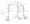
\includegraphics[width=0.6\textwidth]{general_parallel_mechanism.pdf}
    \captionof{figure}{General Parallel Mechanism with Multiple Open Chains \cite{lynch2017modern}}
    \label{fig:general_parallel_mechanism}
    \end{center}
    
    \subsubsection*{Kinematic Formulation}
    
    Let the configuration of the moving platform be given by $T_{sb} \in SE(3)$. Denote the forward kinematics of each chain by $T_i(q_i)$, where $q_i$ represents the joint variables for the $i$-th chain.
    
    \subsubsection*{Loop-Closure Conditions}
    
    The loop-closure conditions can be written as:
    
    \begin{equation}
    T_{sb} = T_1(q_1) = T_2(q_2) = \cdots = T_n(q_n)
    \end{equation}
    
    \subsubsection*{Constraint Equations}
    
    By equating the transformations, we obtain a set of constraint equations. The number of independent equations determines the degrees of freedom of the mechanism.
    
    \subsubsection*{Forward and Inverse Kinematics}
    
    The forward and inverse kinematics problems involve solving these constraint equations for unknown joint variables or the platform configuration, respectively.
    
    \subsection*{Application to the Slider-Crank Linkage}
    
    Now, let's apply this general approach to the specific slider-crank linkage of type 1-RRPR shown in Figure 3.
    
    \begin{center}
    
\includegraphics[width=0.6\textwidth]{slider_crank_linkage.pdf}
    \captionof{figure}{Slider-crank linkage (1-RRPR)}
    \label{fig:slider_crank}
    \end{center}
    
    \subsubsection*{Forward Kinematics Analysis}

The forward kinematics of the slider-crank linkage (1-RRPR) was analyzed using a symbolic computation approach. The analysis yielded the following results:

\paragraph{Method:} The mechanism was modeled using two kinematic chains and a loop-closure condition was applied to ensure that both chains meet at the same point.

\paragraph{Results:} The forward kinematics solution provides two possible configurations for the output joint angle $q_1$ in terms of the input prismatic joint displacement $q_3$:

\begin{equation}
q_1 = \begin{cases}
    2\arctan\left(\sqrt{\frac{l_1^2 + 2l_1l_2 + l_2^2 - q_3^2}{-l_1^2 + 2l_1l_2 - l_2^2 + q_3^2}}\right) \\[10pt]
    -2\arctan\left(\sqrt{\frac{-l_1^2 + 2l_1l_2 + l_2^2 - q_3^2}{l_1^2 - 2l_1l_2 + l_2^2 - q_3^2}}\right)
\end{cases}
\end{equation}

where:
\begin{itemize}
    \item $q_1$ is the output joint angle (revolute)
    \item $q_3$ is the input prismatic joint displacement
    \item $l_1$ and $l_2$ are the lengths of the first and second links, respectively
\end{itemize}

\paragraph{Interpretation:}
\begin{itemize}
    \item The two solutions represent the two possible configurations of the mechanism for a given input $q_3$.
    \item The first solution corresponds to the "elbow-up" configuration.
    \item The second solution corresponds to the "elbow-down" configuration.
    \item The solutions involve the ratio of differences of squared lengths, reflecting the geometric constraints of the mechanism.
\end{itemize}

\paragraph{Limitations:}
\begin{itemize}
    \item The expressions under the square roots must be non-negative for real solutions to exist. This condition defines the feasible workspace of the mechanism.
    \item The solution assumes $l_1^2 - 2l_1l_2 + l_2^2 - q_3^2 \neq 0$ and $-l_1^2 + 2l_1l_2 - l_2^2 + q_3^2 \neq 0$. When these conditions are not met, the mechanism is in a singular configuration.
    \item The arctan function should be implemented as atan2 in most programming languages to handle all quadrants correctly.
\end{itemize}

\paragraph{Geometric Interpretation:}
The solutions can be interpreted geometrically:
\begin{itemize}
    \item The numerator $l_1^2 + 2l_1l_2 + l_2^2 - q_3^2$ represents the square of the sum of the link lengths minus the square of the input displacement.
    \item The denominator $-l_1^2 + 2l_1l_2 - l_2^2 + q_3^2$ represents the square of the difference of the link lengths minus the square of the input displacement.
    \item The ratio of these terms, when square-rooted, gives the tangent of half the output angle, which is then doubled to get the full angle.
\end{itemize}

This forward kinematics solution provides a comprehensive understanding of the slider-crank mechanism's behavior, allowing for the prediction of the output angle given the input displacement. The form of the solution highlights the nonlinear nature of the mechanism's kinematics and the importance of considering multiple solutions in parallel mechanisms.

\paragraph{Detailed Calculations:} The complete derivation and step-by-step calculations for the forward kinematics can be found in the Jupyter notebook \texttt{E5.ipynb} located in the Code folder. This notebook provides a comprehensive breakdown of the symbolic computations, including the definition of the kinematic chains, application of the loop-closure condition, and the solution process for obtaining these forward kinematics expressions.
    
    \subsubsection*{2. Inverse Kinematics}
    
%    Similarly, the expression for inverse kinematics, $q_3 = f^{-1}(q_1)$, is derived as:
%    
%    \begin{equation}
%    q_3 = \sqrt{L_1^2 + L_2^2 - 2L_1L_2\cos(q_1)}
%    \end{equation}
    
The inverse kinematics of the slider-crank linkage (1-RRPR) was analyzed using python's symbolic computation with Symforce \cite{martiros2022symforce} \paragraph{Detailed Calculations:} The complete derivation and step-by-step calculations for the forward kinematics can be found in the Jupyter notebook \texttt{E5.ipynb} located in the Code folder. This notebook provides a comprehensive breakdown of the symbolic computations, including the definition of the kinematic chains, application of the loop-closure condition, and the solution process for obtaining the forward kinematics expressions. The analysis yielded the following results:

\paragraph{Method:} The inverse kinematics problem involves finding the input prismatic joint displacement $q_3$ given the output revolute joint angle $q_1$. The solution was derived using the loop-closure condition and solving the resulting equations.

\paragraph{Results:} The inverse kinematics solution provides two possible configurations for the input prismatic joint displacement $q_3$ in terms of the output joint angle $q_1$:

\begin{equation}
q_3 = \begin{cases}
    -\frac{l_2 \sin(q_1)}{\sin(2\alpha_1)} \\[10pt]
    \frac{l_2 \sin(q_1)}{\sin(2\alpha_2)}
\end{cases}
\end{equation}

where:
\begin{align*}
\alpha_1 &= \arctan\left(-\frac{l_1} {\sin(q_1)l_2} + \frac{1}{\tan(q_1)} + \frac{\sqrt{l_1^2 - 2l_1l_2\cos(q_1) + l_2^2}}{l_2 \sin(q_1)}\right) \\[10pt]
\alpha_2 &= \arctan\left(-\frac{l_1} {\sin(q_1)l_2} - \frac{1}{\tan(q_1)} + \frac{\sqrt{l_1^2 - 2l_1l_2\cos(q_1) + l_2^2}}{l_2 \sin(q_1)}\right)
\end{align*}

and:
\begin{itemize}
    \item $q_1$ is the output joint angle (revolute)
    \item $q_3$ is the input prismatic joint displacement
    \item $l_1$ and $l_2$ are the lengths of the first and second links, respectively
\end{itemize}

\paragraph{Interpretation:}
\begin{itemize}
    \item The two solutions represent the two possible configurations of the mechanism for a given output angle $q_1$.
    \item The solutions involve complex trigonometric expressions, reflecting the nonlinear nature of the mechanism's kinematics.
    \item The $\alpha_1$ and $\alpha_2$ terms represent intermediate angles in the mechanism's configuration.
    \item The solution depends on the ratio of trigonometric functions of these intermediate angles to $l_2 \sin(q_1)$, which relates to the mechanism's geometry.
\end{itemize}

\paragraph{Limitations and Considerations:}
\begin{itemize}
    \item The solution assumes $\sin(q_1) \neq 0$. When $\sin(q_1) = 0$ (i.e., $q_1 = 0$ or $\pi$), the mechanism is in a singular configuration.
    \item The expressions under the square roots must be non-negative for real solutions to exist. This condition defines the feasible workspace of the mechanism.
    \item The arctan function should be implemented as atan2 in most programming languages to handle all quadrants correctly.
    \item Numerical stability should be considered when implementing these solutions, especially near singular configurations.
\end{itemize}


    
\subsubsection*{4. Maximum Output Angular Velocity}

To find an expression for the maximum output angular velocity $\dot{q}_{1max}$ given the maximum velocity $\dot{q}_{3max}$ available at the actuator, we used symbolic computation in the Jupyter notebook E5.ipynb. The process and results are as follows:

\paragraph{Method:}
\begin{itemize}
	\item We defined time-dependent variables for $q_1$, $q_2$, $q_3$, and $l_2$.
	\item Using the forward kinematics solutions, we calculated the Jacobians $\frac{\partial q_1}{\partial q_3}$ for both solutions.
	\item The maximum output angular velocity was then calculated as $\dot{q}_{1max} = |\frac{\partial q_1}{\partial q_3}| \cdot \dot{q}_{3max}$.
\end{itemize}

\paragraph{Results:}
The symbolic computation yielded the following expressions for $\dot{q}_{1max}$:

For both solutions:

\begin{equation} \label{eq:jacob1}
\dot{q}_{1max}=2\dot{q}_{3max}\left|\frac{q_3(t)\cdot \sqrt{\frac{l_1^2 - 2l_1l_2(t) + l_2^2(t) - q_3^2(t)}{l_1^2 + 2l_1l_2(t) + l_2^2(t) - q_3^2(t)}}}{ {l_1^2 - 2l_1l_2(t) + l_2^2(t) - q_3^2(t)}} \right|
\end{equation}

\paragraph{Interpretation:}
\begin{itemize}
	\item The expression for $\dot{q}_{1max}$ is the same for both solutions of the forward kinematics, indicating that the maximum output angular velocity is independent of which configuration the mechanism is in.
	\item The maximum output angular velocity depends on the current state of the mechanism (represented by $q_3(t)$ and $l_2(t)$) and the geometric parameters ($l_1$).
	\item The expression involves ratios of quadratic terms in $q_3(t)$ and $l_2(t)$, reflecting the nonlinear nature of the mechanism's kinematics.
	\item The absolute value in the expression ensures that $\dot{q}_{1max}$ is always positive, as it represents a magnitude.
\end{itemize}

\paragraph{Limitations and Considerations:}
\begin{itemize}
	\item The expression becomes undefined when $l_1^2 - 2l_1l_2(t) + l_2^2(t) - q_3^2(t) = 0$, which corresponds to a singular configuration of the mechanism.
	\item The time dependence of $l_2$ ($l_2(t)$) in the derived expression suggests that the analysis considered potential variations in link lengths, which might not be applicable in a rigid mechanism. For a fixed-length mechanism, $l_2$ would be constant.
	\item The actual maximum velocity achievable may be lower due to physical constraints not captured in this kinematic analysis, such as joint limits or dynamic effects.
\end{itemize}

\paragraph{Detailed Calculations:}
The complete derivation, including the symbolic manipulation and intermediate steps, can be found in the Jupyter notebook E5.ipynb in the Code folder. This notebook provides a step-by-step breakdown of the calculation process using the SymForce library for symbolic mathematics.
    
\subsubsection*{5. Maximum Output Torque}

Given that the maximum force available at the actuator (prismatic joint q3) is $f_{max}$, we need to find an expression for the maximum output torque $\tau_{max}$ at the revolute joint q1.

To derive this relationship, we use the principle of virtual work and the Jacobian of the mechanism.

\paragraph{Method:}
\begin{itemize}
    \item Let $J$ be the Jacobian that relates the velocity of q3 to the angular velocity of q1: $\dot{q}_1 = J \dot{q}_3$
    \item By the principle of virtual work, we have: $\tau_1 \delta q_1 = f_3 \delta q_3$
    \item Substituting $\delta q_1 = J \delta q_3$, we get: $\tau_1 J \delta q_3 = f_3 \delta q_3$
    \item This implies: $\tau_1 = \frac{f_3}{J}$
\end{itemize}

\paragraph{Expression for Maximum Output Torque:}
Given the maximum force $f_{max}$ at the actuator, the maximum output torque is:

\begin{equation}
    \tau_{max} = \frac{f_{max}}{J} = f_{max} \cdot \frac{1}{J}
\end{equation}

where $J$ is the Jacobian we derived earlier \eqref{eq:jacob1}:

\begin{equation}
    J = 2\left|\frac{q_3(t)\cdot \sqrt{\frac{l_1^2 - 2l_1l_2(t) + l_2^2(t) - q_3^2(t)}{l_1^2 + 2l_1l_2(t) + l_2^2(t) - q_3^2(t)}}}{ {l_1^2 - 2l_1l_2(t) + l_2^2(t) - q_3^2(t)}} \right|
\end{equation}

Substituting this into our expression for $\tau_{max}$:

\begin{equation}
    \tau_{max} = 2f_{max}\cdot\left|\frac{ {l_1^2 - 2l_1l_2(t) + l_2^2(t) - q_3^2(t)}}{q_3(t)\cdot \sqrt{\frac{l_1^2 - 2l_1l_2(t) + l_2^2(t) - q_3^2(t)}{l_1^2 + 2l_1l_2(t) + l_2^2(t) - q_3^2(t)}}} \right|
\end{equation}

\paragraph{Interpretation:}
\begin{itemize}
    \item The maximum output torque $\tau_{max}$ is directly proportional to the maximum force $f_{max}$ available at the actuator.
    \item $\tau_{max}$ depends on the current state of the mechanism (represented by $q_3(t)$ and $l_2(t)$) and the geometric parameters ($l_1$).
    \item The expression involves ratios of quadratic terms in $q_3(t)$ and $l_2(t)$, reflecting the nonlinear nature of the mechanism's kinematics.
    \item $\tau_{max}$ is inversely proportional to the Jacobian, meaning it increases when the mechanism is in configurations that provide mechanical advantage.
\end{itemize}

\paragraph{Limitations and Considerations:}
\begin{itemize}
    \item This analysis assumes static conditions and doesn't account for dynamic effects.
    \item The expression becomes undefined when $l_1^2 - 2l_1l_2(t) + l_2^2(t) - q_3^2(t) = 0$, which corresponds to a singular configuration of the mechanism.
    \item The time dependence of $l_2$ ($l_2(t)$) in the derived expression suggests that the analysis considered potential variations in link lengths, which might not be applicable in a rigid mechanism. For a fixed-length mechanism, $l_2$ would be constant.
    \item In practice, joint limits and other mechanical constraints may prevent reaching the theoretical maximum torque in certain configurations.
\end{itemize}

The detailed derivation and symbolic manipulation can be found in the Jupyter notebook \texttt{E5.ipynb} in the Code folder.    \end{solution}
\subsection{6. singular configurations}
Here we will Identify any singular configurations of the slider-crank mechanism.

\begin{solution}
    The slider-crank mechanism (1-RRPR) has several singular configurations. These configurations can be identified by analyzing the Jacobian of the mechanism and finding positions where it becomes rank-deficient. The singular configurations are:

    \begin{enumerate}
        \item \textbf{Fully Extended Configuration:}
        \begin{itemize}
            \item When $q_1 = 0$ or $\pi$
            \item In this configuration, the two links are fully extended or folded
            \item The mechanism loses the ability to transmit force/motion in the direction perpendicular to the links
        \end{itemize}

        \item \textbf{Maximum Extension of Prismatic Joint:}
        \begin{itemize}
            \item When $q_3 = l_1 + l_2$
            \item The prismatic joint is at its maximum extension
            \item The mechanism loses the ability to extend further
        \end{itemize}

        \item \textbf{Minimum Extension of Prismatic Joint:}
        \begin{itemize}
            \item When $q_3 = |l_1 - l_2|$
            \item The prismatic joint is at its minimum extension
            \item The mechanism loses the ability to contract further
        \end{itemize}
    \end{enumerate}

    In these configurations, the mechanism loses one or more degrees of freedom, and the relationship between input and output velocities becomes indeterminate. These singularities are important to consider in the design and control of the mechanism, as they can lead to loss of control or excessive forces in the joints.

    \paragraph{Note:} The Jacobian analysis leading to the identification of these singular configurations can be found in the Jupyter notebook \texttt{E5.ipynb} in the Code folder.
\end{solution}


\subsection{Exercise 6}
Donald is from the United States of America and Angela comes from Europe. They have to work together on a robotics project and they don't always agree with each other. While Donald is obsessed with the Imperial system of units, Angela likes to use the modern metric system. They are together working on a 6 DOF robotic manipulator (with 3 translational and 3 rotational DOFs) mounted on a 3 DOF gantry crane which can place the base of the robot in any 3D position $(x_B, y_B, z_B) \in \mathbb{R}^3$. Angela develops the software for the robot manipulator and Donald develops the software for the 3 DOF gantry crane. They are exchanging black-box models and are not allowed to modify each other's code.

\begin{solution}

\subsubsection*{1. Converting meters to inches for the gantry crane}

Yes, Angela can find a linear scaling factor to convert the 3D position from meters to inches.

\begin{itemize}
    \item The conversion factor from meters to inches is: 1 meter = 39.3701 inches
    \item This is a constant scalar value that can be applied uniformly to all three dimensions
    \item The conversion can be represented as a linear transformation:
    
    \begin{equation}
        \begin{bmatrix} x_{\text{inches}} \\ y_{\text{inches}} \\ z_{\text{inches}} \end{bmatrix} = 
        39.3701 \cdot \begin{bmatrix} x_{\text{meters}} \\ y_{\text{meters}} \\ z_{\text{meters}} \end{bmatrix}
    \end{equation}
\end{itemize}

This linear scaling preserves the proportions and relationships in the 3D space, making it suitable for use with Donald's model.

\subsubsection*{2. Converting metric to imperial for the robot manipulator}

Donald cannot use a single linear scaling factor to convert the 6D pose from the metric system to the imperial system.

\begin{itemize}
    \item For the translational part $(x_E, y_E, z_E)$, a linear scaling factor (39.3701) can be used to convert from meters to inches, similar to part 1.
    \item However, for the rotational part:
    \begin{itemize}
        \item Quaternions cannot be directly converted to Euler angles (roll, pitch, yaw) using a linear scaling factor.
        \item The conversion from quaternions to Euler angles involves nonlinear trigonometric functions.
        \item Even after converting to Euler angles, no scaling is needed as angles are dimensionless (radians to degrees conversion is a simple multiplication by $180/\pi$, but this is not related to the metric-imperial conversion).
    \end{itemize}
\end{itemize}

Therefore, a single linear scaling factor cannot be applied to the entire 6D pose to achieve the desired conversion.

\subsubsection*{3. Using each other's models}

Yes, it is possible for Donald and Angela to use each other's models with some additional steps:

\begin{itemize}
    \item For Donald to use Angela's inverse kinematics model:
    \begin{itemize}
        \item Convert translational inputs from inches to meters: multiply by 1/39.3701
        \item Convert rotational inputs from Euler angles (degrees) to quaternions
        \item Apply Angela's model
        \item No conversion needed for the output (actuator commands)
    \end{itemize}
    
    \item For Angela to use Donald's gantry crane model:
    \begin{itemize}
        \item Convert inputs from meters to inches: multiply by 39.3701
        \item Apply Donald's model
        \item No conversion needed for the output (actuator commands)
    \end{itemize}
\end{itemize}

These conversions can be implemented as wrapper functions around the black-box models, allowing Donald and Angela to work in their preferred units while still utilizing each other's software components effectively.

\end{solution}


\section{Dynamics}
\subsection{Exercise 7}
Consider a pendulum robot with a bob of mass $m$ connected to the ground link by a massless link of length $l$ in Figure 4. Denote with $\theta$ the angle made by the bob with the vertical axis in the anti-clockwise sense.

\begin{solution}

\subsubsection*{1. Inverse Dynamics}

The expression for torque acting at the revolute joint ($\tau$) in terms of ($\theta$, $\dot{\theta}$, $\ddot{\theta}$) is:

\begin{equation}
    \tau = ml^2\ddot{\theta} + mgl\sin(\theta)
\end{equation}

where:
\begin{itemize}
    \item $m$ is the mass of the bob
    \item $l$ is the length of the link
    \item $g$ is the acceleration due to gravity
    \item $\theta$, $\dot{\theta}$, and $\ddot{\theta}$ are the angular position, velocity, and acceleration respectively
\end{itemize}

This equation accounts for both the inertial torque ($ml^2\ddot{\theta}$) and the gravitational torque ($mgl\sin(\theta)$).

\subsubsection*{2. Forward Dynamics}

The expression for acceleration at the revolute joint ($\ddot{\theta}$) in terms of ($\tau$) is:

\begin{equation}
    \ddot{\theta} = \frac{\tau - mgl\sin(\theta)}{ml^2}
\end{equation}

This equation is derived by solving the inverse dynamics equation for $\ddot{\theta}$.

\subsubsection*{3. Simulation Program}

To simulate the free-fall of the pendulum (i.e., $\tau = 0.0$), we can use a simple Newton-Euler numerical integration scheme. Here's a Python program that implements this simulation and provides a visualization:

\begin{verbatim}
import numpy as np
import matplotlib.pyplot as plt
from matplotlib.animation import FuncAnimation

# Parameters
m = 1.0  # mass of bob (kg)
l = 1.0  # length of pendulum (m)
g = 9.81  # acceleration due to gravity (m/s^2)
dt = 0.01  # time step (s)
t_max = 10.0  # maximum simulation time (s)

# Initial conditions
theta = np.pi/4  # initial angle (radians)
omega = 0.0  # initial angular velocity (rad/s)

# Lists to store simulation data
t_list = [0]
theta_list = [theta]

# Simulation loop
t = 0
while t < t_max:
    # Calculate acceleration
    alpha = -g/l * np.sin(theta)
    
    # Update angular velocity and position
    omega += alpha * dt
    theta += omega * dt
    
    # Store results
    t += dt
    t_list.append(t)
    theta_list.append(theta)

# Convert lists to numpy arrays
t_array = np.array(t_list)
theta_array = np.array(theta_list)

# Calculate x and y positions of the bob
x = l * np.sin(theta_array)
y = -l * np.cos(theta_array)

# Create animation
fig, ax = plt.subplots()
ax.set_xlim(-l-0.1, l+0.1)
ax.set_ylim(-l-0.1, l+0.1)
line, = ax.plot([], [], 'o-', lw=2)

def init():
    line.set_data([], [])
    return line,

def animate(i):
    line.set_data([0, x[i]], [0, y[i]])
    return line,

anim = FuncAnimation(fig, animate, init_func=init,
                     frames=len(t_array), interval=dt*1000, blit=True)

plt.show()
\end{verbatim}

This program uses the forward dynamics equation with $\tau = 0$ to simulate the free-fall of the pendulum. It employs a simple Euler integration method to update the pendulum's state over time. The resulting animation shows the pendulum swinging back and forth under the influence of gravity.

Key components of the simulation:
\begin{itemize}
    \item The acceleration is calculated using $\ddot{\theta} = -\frac{g}{l}\sin(\theta)$ (derived from setting $\tau = 0$ in the forward dynamics equation).
    \item The angular velocity and position are updated using Euler integration.
    \item The position of the bob is calculated in Cartesian coordinates for visualization.
    \item Matplotlib's FuncAnimation is used to create an animation of the pendulum's motion.
\end{itemize}

This simulation provides a visual representation of the pendulum's behavior, allowing for intuitive understanding of its dynamics under free-fall conditions.

\end{solution}

\subsection{Exercise 8}
\lipsum[15]

\begin{solution}
    \lipsum[16]
\end{solution}

\subsection{Exercise 9}
\lipsum[17]

\begin{solution}
    \lipsum[18]
\end{solution}
